\chapter{System Architecture}
\label{chap:architecture}

This chapter presents the Gateway Dashboard system architecture at a high level, focusing on how the key components interact and the design decisions that enable the platform to scale and evolve. Section~\ref{sec:arch_overview} introduces the three tier system architecture and the organisation of backend modules. Section~\ref{sec:tech_stack} describes the technology stack and caching strategy. Section~\ref{sec:database_design} covers the database schema design and entity relationships.

\section{Overview}
\label{sec:arch_overview}

The Gateway Dashboard system follows a modern three tier architecture designed for clarity, scalability, and maintainability. The system separates concerns across three distinct layers: a user facing frontend built with Vue.js, a business logic layer implemented in NestJS, and a persistent data layer comprising MongoDB and Redis. This separation allows each layer to evolve independently while maintaining clear, well defined communication boundaries.

\subsection{Three-Tier Architecture}

Figure~\ref{fig:system_three_tier} illustrates the three tier architecture and the external services integrated into the system.

\begin{figure}[H]
\centering
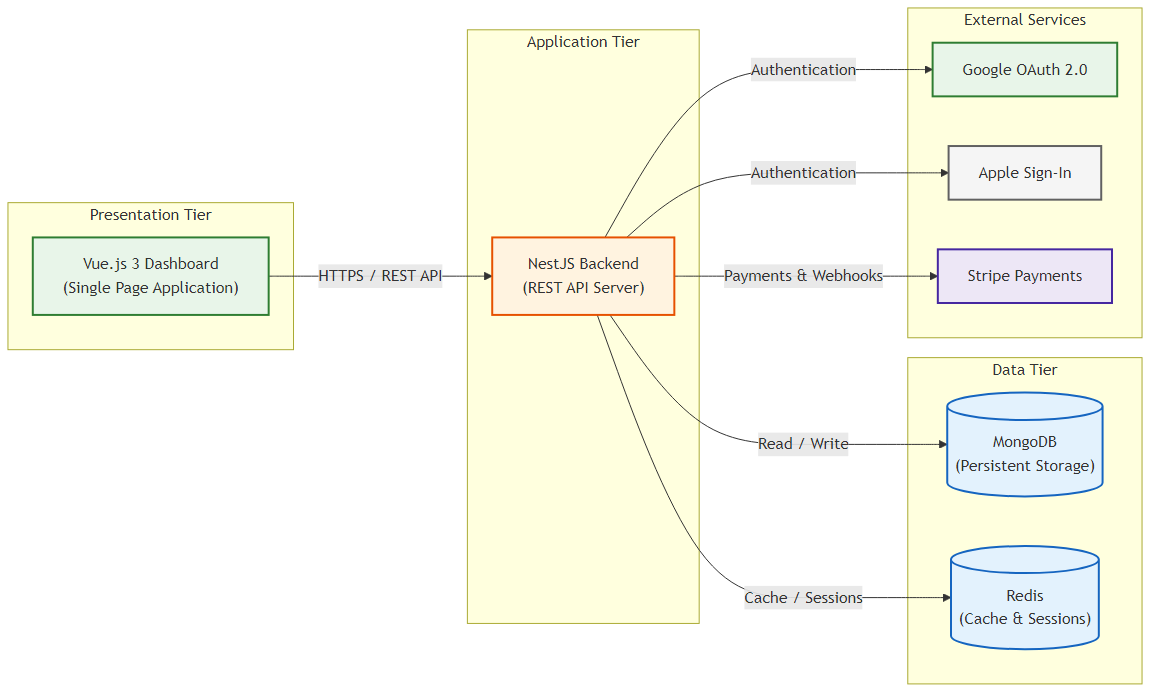
\includegraphics[width=0.85\textwidth]{images/system_three_tier.png}
\caption{Three-Tier System Architecture}
\label{fig:system_three_tier}
\end{figure}

The \textbf{Presentation Tier} is a Single Page Application built with Vue.js 3, running entirely in the user's browser. It communicates with the backend through standard HTTPS REST API calls. The \textbf{Application Tier} is a NestJS server that processes all business logic, including authentication, payment handling, and subscription management. The \textbf{Data Tier} uses MongoDB for persistent storage of user accounts, subscriptions, and plan definitions, alongside Redis for caching frequently accessed data and managing user sessions.

Three external services are integrated: \textbf{Google OAuth 2.0} and \textbf{Apple Sign-In} provide SSO authentication, while \textbf{Stripe} handles all payment processing and sends real time event notifications back to the backend via webhooks.

\subsection{Backend Module Organisation}

Figure~\ref{fig:backend_modules} shows how the backend is organised into distinct modules, each responsible for a specific area of functionality.

\begin{figure}[H]
\centering
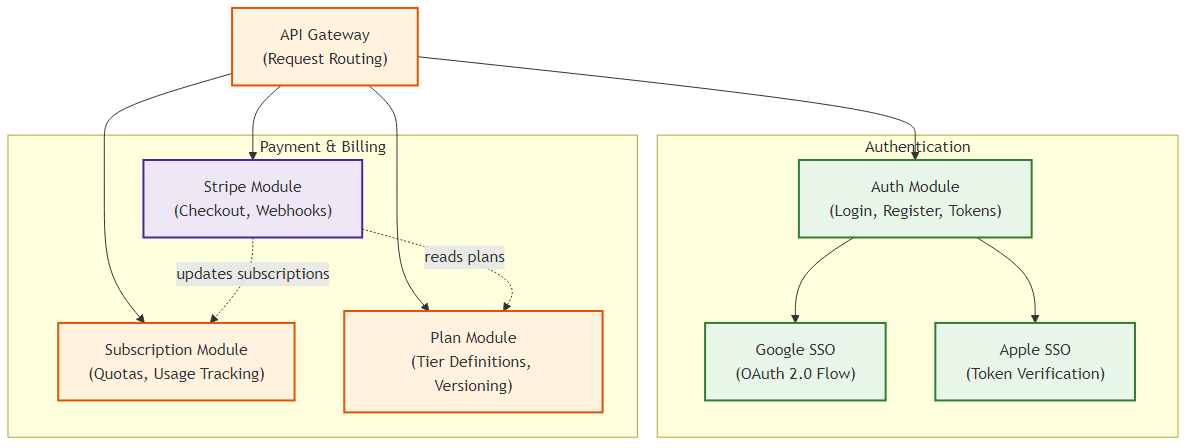
\includegraphics[width=0.75\textwidth]{images/backend_modules.png}
\caption{Backend Module Organisation}
\label{fig:backend_modules}
\end{figure}

The API Gateway routes incoming requests to the appropriate module. The \textbf{Authentication} group handles user login, registration, and token management, with dedicated submodules for Google SSO (using the OAuth 2.0 redirect flow) and Apple SSO (using token verification). The \textbf{Payment \& Billing} group consists of the Stripe Module (which manages checkout sessions and processes payment webhooks), the Subscription Module (which tracks each user's subscription status and usage quotas), and the Plan Module (which stores versioned plan definitions and caches them for performance). The dotted lines indicate cross module communication: the Stripe Module reads plan definitions when creating checkout sessions and updates subscription records when payment events occur.

\subsection{Communication Flow}

User interactions flow naturally through the system: when a user interacts with the frontend, the browser sends HTTP requests to the backend API, where incoming requests are validated and authorised. The backend then executes the required business logic, which may involve retrieving or storing data, checking cached values, or communicating with external payment and authentication services. Once processing is complete, the backend responds with the result, allowing the frontend to update the user interface accordingly.

\input{tex/ch3_architecture/02_tech_stack}
\section{Database Design}
\label{sec:database_design}

The database schema is designed to support user account management, secure authentication, subscription tracking, and flexible service plan versioning. MongoDB's document-oriented approach provides the flexibility needed for an evolving application while maintaining data consistency and relationships.

\subsection{Core Data Model}

The system manages several interconnected data domains. The \textbf{Users} collection is the foundation, storing user account information including email, authentication credentials, user roles, and subscription status. Each user account can have an associated \textbf{Subscription}, which tracks their current service plan, usage quotas, and billing integration with external payment systems. The \textbf{Plans} collection maintains versioned service offerings, allowing the business to introduce new plans or modify existing ones without disrupting active subscriptions.

To support secure session management, two additional collections manage authentication state. The \textbf{UserTokens} collection tracks active authentication tokens for each user session, storing metadata such as token expiration time and client information. The \textbf{TokenBlacklist} collection maintains a record of revoked tokens, ensuring that logged-out users or users with invalidated sessions cannot reuse their old authentication credentials. Both collections leverage MongoDB's automatic expiration (TTL) feature to clean up old entries without manual intervention.

\subsection{Entity Relationships}

Figure~\ref{fig:er_diagram} illustrates how these collections relate to one another:

\begin{figure}[H]
\centering
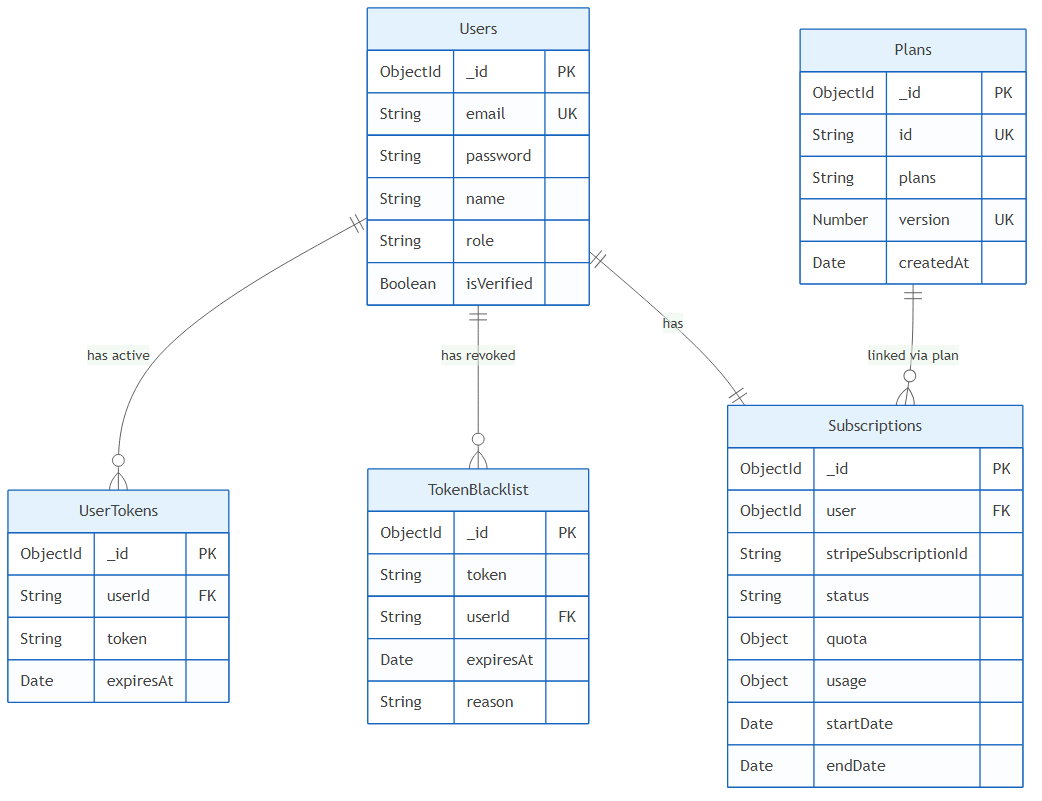
\includegraphics[width=0.75\textwidth]{images/er_diagram.png}
\caption{Entity Relationship Diagram}
\label{fig:er_diagram}
\end{figure}

The data model reflects common business logic. Each user maintains at most one active subscription, creating a one-to-one relationship. A subscription references an available plan and integrates with Stripe to track billing information. Users may have multiple active authentication tokens (for different devices or sessions), creating a one-to-many relationship. When users log out or sessions are invalidated, their tokens are moved to the blacklist to prevent reuse. The Plans collection exists independently but is logically referenced by subscriptions, enabling the application to manage plan availability and pricing changes without affecting existing customer data.

\subsection{Design Decisions}

The database schema reflects several key design principles. By storing user account information, subscription details, and authentication tokens in separate collections, the schema maintains clean separation of concerns—account data, billing data, and session management can be queried and updated independently. The use of document-based storage allows subscription records to embed service quota and usage information, making it efficient to retrieve complete subscription details in a single database operation. Token expiration handling through TTL indexes eliminates the need for periodic cleanup jobs, reducing operational complexity. This design balances normalization (separating logically distinct concepts) with denormalization (embedding related data to minimize joins), a practical approach for document databases like MongoDB.


\section{Summary}

This chapter presented the Gateway Dashboard system architecture across three layers. The three tier design separates the Vue.js frontend, NestJS backend, and MongoDB/Redis data layer, allowing each to evolve independently. The backend is organised into modular components for authentication (with Google and Apple SSO), payment processing (via Stripe), and subscription management, communicating through well defined interfaces. The technology stack leverages industry standard frameworks chosen for reliability, developer experience, and scalability. The database schema uses MongoDB's document oriented approach with separate collections for users, subscriptions, plans, tokens, and token blacklisting, supported by Redis caching to reduce latency on frequently accessed data. Together, these architectural decisions provide a solid foundation for the implementation described in the next chapter.
